\chapter{Modelli a rete elastica}
\section{Fluttuazioni dello stato nativo}
Dopo aver compiuto il processo di ripiegamento, la proteina non risulta statica in quanto gli atomi che la compongono sono soggetti a fluttuazioni termiche. 
Come già detto, lo stato nativo rappresenta un minimo dell'energia e di conseguenza le fluttuazioni termiche inducono delle variazioni nella struttura proteica che oscillerà attorno a questo. 
In un intorno del minimo dell'energia si viene quindi a formare un \textit{ensemble} di microstati che si trovano in equilibrio dinamico. Un esempio di quanto accade per una determinata struttura proteica è raffigurato in Figura~\ref{fig:microstates} dove si vede come nel minimo dell'energia dello stato nativo, osservando ad una maggiore risoluzione, si possano riconoscere due differenti sottostati, i quali a loro volta sono costituiti da microstati, riscontrabili ad una risoluzione ancora maggiore. 
Queste variazioni non influiscono sulle strutture secondarie e terziarie ma provocano uno spostamento dei singoli atomi che può essere osservato in termini di alterazioni della lunghezza dei legami e dei loro angoli, della conformazione dei loop e della posizione e orientazione di interi domini o sottounità proteiche. \cite{chem_rev}
\begin{figure}[h]
	\centering
	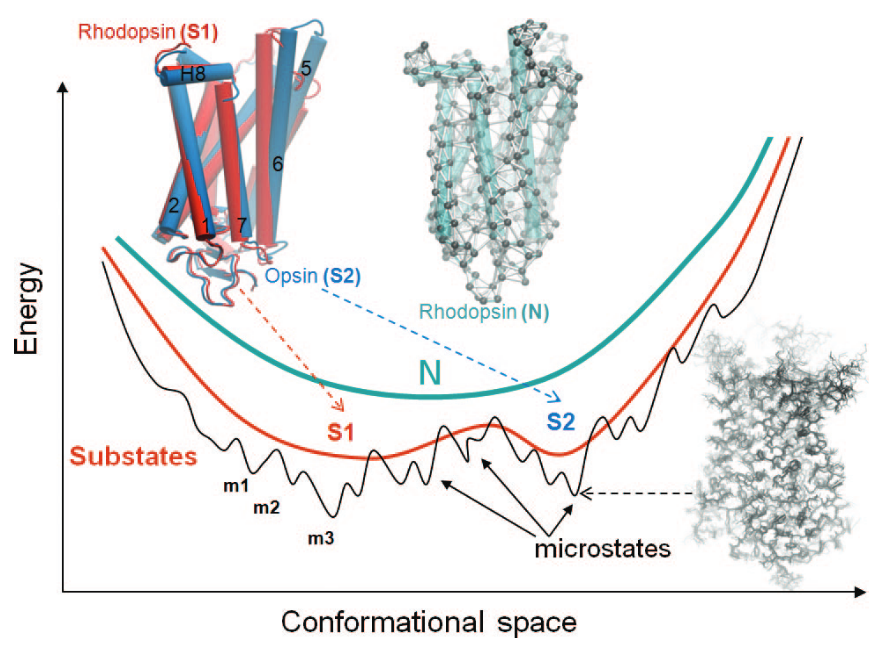
\includegraphics[width=11cm]{/home/michele_puppin/Scrivania/stesura_tesi/immagini/microstates.png}
	\caption{Profilo energetico dello stato nativo a differenti risoluzioni \cite{chem_rev}}
	\label{fig:microstates}
\end{figure}

Per lo studio di questi fenomeni si ricorre a metodi di \textit{principal component analysis} (PCA), come ad esempio analisi ai modi normali, dinamica molecolare e simulazioni Monte Carlo.
Tramite questi è stato possibile verificare come queste fluttuazioni non siano affatto casuali ma inducano movimenti collettivi e coordinati che sono quindi rilevanti da un punto di vista funzionale.
Svolgono importanti funzioni biologiche in quanto non si limitano a rendere possibili i movimenti dei domini e delle sottounità proteiche ma li conducono e li coordinano attivamente. Risultano fondamentali nello svolgimento delle funzioni di catalisi e in particolare nella regolazione allosterica, rendendo possibile il legame con il substrato. La funzioni delle proteine di membrana, ad esempio, che svolgono attività di trasmissione dei segnali, apertura dei pori e trasferimento degli ioni, sono rese possibili da questi moti collettivi.
La rilevanza delle fluttuazioni evidenzia come la loro presenza sia necessariamente dovuta alla struttura stessa della proteina. La dinamica all'equilibrio risulta influenzata dalla struttura della proteina analogamente alla determinazione dello stato nativo a partire dalla sequenza di amminoacidi. Questi movimenti collettivi sono quindi codificati nella struttura tridimensionale e di conseguenza nella topologia dello stato nativo. \cite{chem_rev} 

\section{Analisi ai modi normali}
L'analisi ai modi normali (NMA) è tra i metodi PCA più utilizzati. 
In questo metodo si assume che le fluttuazioni attorno allo stato nativo, dovute all'agitazione termica, siano governate da un potenziale armonico al fine di studiare i modi normali di oscillazione. Data la scelta del potenziale, questo metodo risulta valido in prossimità dell'equilibrio dove l'effettivo potenziale a cui sono soggetti gli atomi della proteina può essere approssimato con quello armonico. Si trascurano quindi altri vincoli che la struttura proteica impone alle deformazioni, come ad esempio la lunghezza dei legami o gli angoli di legame, e questo contribuisce a rendere l'assunzione del potenziale valida unicamente in prossimità dell'equilibrio. 
L'analisi ai modi normali risulta dunque utile sopratutto per lo studio di variazioni della configurazione che avvengono su larga scala in quanto le specifiche interazioni locali, in particolare quelle di natura elettromagnetica, non sono prese in considerazione.
Questo tipo di variazioni, indicate come modi globali, sono di notevole interesse poiché sono quelle che risultano biologicamente funzionali. I modi globali rappresentano le riconfigurazioni lungo le direzioni più facilmente accessibili energeticamente in quanto richiedono la minima quantità di energia per dar luogo ad una data deformazione. \cite{chem_rev}

Si considera una proteina con $ N $ residui e si assume che per ognuno di questi il centro di interazione del potenziale risieda nel carbonio $ \mathrm{C}^{\alpha} $. Per ognuna delle possibili configurazioni, si associa al carbonio $ \mathrm{C}^{\alpha} $ del residuo $ i $-esimo un vettore posizione $ \mathbf{R}_{i} = (x_{i}, \; y_{i}, \; z_{i})^{\mathrm{T}} $. 
Il vettore associato alla configurazione può quindi essere scritto come
\begin{equation}
	\mathbf{q} = ((\mathbf{R}_{1})^{\mathrm{T}}, \; ... \; , \; (\mathbf{R}_{N})^{\mathrm{T}})^{\mathrm{T}} =
	(x_{1}, \; y_{1}, \; z_{1}, \; ... \; , \; x_{N}, \; y_{N}, \; z_{N})^{\mathrm{T}}.
\end{equation}
Una volta indicata con l'apice $ 0 $ la configurazione di equilibrio corrispondente allo stato nativo, è possibile definire il vettore di spostamento $ \Delta \mathbf{q} = \mathbf{q} -  \mathbf{q}^0$ che descrive la variazione della posizione $ \Delta \mathbf{R}_{i} = \mathbf{R}_{i} -  \mathbf{R}^{0}_{i}$ di ognuno degli $ N $ siti.
Se l'interazione è dominata da un potenziale $ V $, questo può essere espanso come serie di potenze di $ \mathbf{q}  $ vicino all'equilibrio
\begin{equation}
	V(\mathbf{q}) =  V(\mathbf{q}^0) + \sum_i \left( \frac{\partial V}{\partial q_i} \right)^0 (q_i - q^{0}_{i}) + \frac{1}{2} \sum_{ij} \left( \frac{\partial^2 V}{\partial q_i \partial q_j} \right)^0 (q_i - q^{0}_{i})(q_j - q^{0}_{j}) + ...
\end{equation}
Il primo termine rappresenta il valore minimo dell'energia e può essere arbitrariamente annullato, mentre il secondo termine deve essere nullo in quanto ci si è posti in una condizione di equilibrio. È possibile quindi riscrivere il potenziale nella forma
\begin{equation}\label{eq:potential}
\begin{split}
	 V(\mathbf{q}) & = \frac{1}{2} \sum_{ij} \left( \frac{\partial^2 V}{\partial q_i \partial q_j} \right)^0 (q_i - q^{0}_{i})(q_j - q^{0}_{j}) \\
 	& =\frac{1}{2} \sum_{ij}  (q_i - q^{0}_{i}) H_{ij} (q_j - q^{0}_{j}) 
 	= \frac{1}{2} \Delta \mathbf{q}^{\mathrm{T}} \mathbf{H} \Delta \mathbf{q}
\end{split} 
\end{equation}
dove si è introdotta la matrice $ \mathbf{H} $ di elementi
\begin{equation} \label{def_mat}
	H_{ij} = \left( \frac{\partial^2 V}{\partial q_i \partial q_j} \right)^0.
\end{equation}
Questa è per costruzione reale e simmetrica. Essendo calcolata a partire da un minimo dell'energia, tutti i suoi autovalori dovranno risultare positivi in quanto rappresentano proprio la curvatura del potenziale e sono positivi per i punti di minimo. È inoltre caratterizzata da sei autovalori nulli che indicano un'assenza di variazione nella configurazione e possono essere quindi associati alle tre traslazioni rigide e alle tre rotazioni rigide.
 
Al fine di studiare la dinamica della configurazione è necessario introdurre la componente di energia cinetica. Se si assume che i siti siano costituiti da particelle di massa $ m $ caratterizzate da un comportamento classico, l'equazione del moto può essere scritta come 
\begin{equation} \label{eq:kinetic}
	\mathbf{M} \frac{\mathrm{d^2} \Delta \mathbf{q}}{\mathrm{d}t^2} +  \mathbf{H} \Delta \mathbf{q} = 0
\end{equation}
dove $ \mathbf{M} $ è una matrice diagonale contenente le masse delle particelle, ognuna ripetuta tre volte. Una soluzione all'equazione (\ref{eq:kinetic}) è fornita dal vettore $ \mathbf{u}_k(t) =  \mathbf{a}_k \exp (-i \omega_k t)$ dove $ \mathbf{a}_k $ è un vettore che contiene l'ampiezza e la fase e $ \omega_k $ rappresenta la frequenza del modo $ k $-esimo. Sostituendo questa soluzione nell'equazione (\ref{eq:kinetic}), l'equazione del moto diventa 
\begin{equation}
	\mathbf{H} \mathbf{u}_k = \omega_{k}^{2} \mathbf{M} \mathbf{u}_k.
\end{equation}
Dopo aver assunto che le masse siano tutte uguali e unitarie, si possono riconoscere nei vettori $ \mathbf{u}_k $ gli autovettori della matrice $ \mathbf{H} $ e in $ \lambda_{k} = \omega_{k}^{2} $ i suoi autovalori.
Si può vedere come per il singolo modo $ k $-esimo, l'equazione (\ref{eq:potential}) può essere riscritta come 
\begin{equation}\label{eq:low_modes}
	V(\mathbf{u}_k) = \frac{1}{2} \mathbf{u}_{k}^{\mathrm{T}} \mathbf{H} \mathbf{u}_{k} = \frac{ \omega_{k}^2}{2}.
\end{equation}
Osservando l'equazione (\ref{eq:low_modes}) si ricava che l'energia è direttamente proporzionale al quadrato della frequenza. I movimenti lungo modi ad alta frequenza sono quindi energeticamente più dispendiosi rispetto a quelli di uguale entità ma lungo modi a bassa frequenza.
Sono proprio questi modi a dare luogo alle deformazioni su larga scala e corrispondono quindi ai modi globali nei quali, come già detto, risiede l'interesse biologico.

\section{Modello anisotropo}
Il punto cruciale dell'analisi ai modi normali consiste nell'individuazione della forma corretta della matrice $ \mathbf{H} $ che è direttamente collegata alla scelta del potenziale.
Per tener conto della complessità delle interazioni all'interno della proteina è possibile scegliere un potenziale semiempirico che prenda in considerazione i differenti contributi. La complessità di potenziali di questo tipo risulta tuttavia problematica in quanto rende necessaria una minimizzazione preliminare dell'energia per assicurare che la derivata prima del potenziale sia nulla. La minimizzazione infatti richiede un elevato sforzo computazionale e produce una configurazione differente dallo stato nativo. 
Si è verificato che scegliendo, invece del potenziale semiempirico, un semplice potenziale elastico, dipendente da un unico parametro, è possibile produrre risultati del tutto analoghi. I risultati prodotti con un potenziale elastico risultano inoltre più accurati grazie alla mancata minimizzazione, al minor numero di parametri nel potenziale e all'assenza di altre problematicità dovute ad una differente scelta del potenziale. 
A rendere efficace questa scelta è il fatto che i modi di interesse sono i modi lenti e coordinati che coinvolgono ampie regioni. Le forze che effettivamente governano questi movimenti sono il risultato della sovrapposizione delle specifiche interazioni che possono essere quindi singolarmente trascurate. \cite{phys_rev}

Per l'analisi ai modi normali si introducono quindi dei modelli a rete elastica (ENM). A partire dalla struttura è possibile modellizzare la proteina costruendo una rete elastica di masse accoppiate a delle molle come raffigurato in Figura~\ref{fig:elastic_network}. La topologia della rete è definita dallo stato nativo e i nodi della rete vengono collegati tramite delle molle qualora la loro distanza reciproca sia inferiore ad un raggio di cutoff prestabilito. Si è visto inoltre che la scelta della costante elastica delle molle ha effetti molto ridotti sui risultati prodotti dall'analisi. \cite{phys_rev}
I principali modelli a rete elastica sono il modello anisotropo (ANM) e il \textit{gaussain network model} (GNM). Quest'ultimo si basa sull'assunzione che le fluttuazioni di ogni residuo siano distribuite in modo gaussiano attorno all'equilibrio e utilizza un potenziale la quale forma fa si che le fluttuazioni siano isotrope. Di conseguenza tale metodo non fornisce informazioni sulle direzioni del moto nei differenti modi. \cite{iop_science}
\begin{figure}[h]
	\centering
	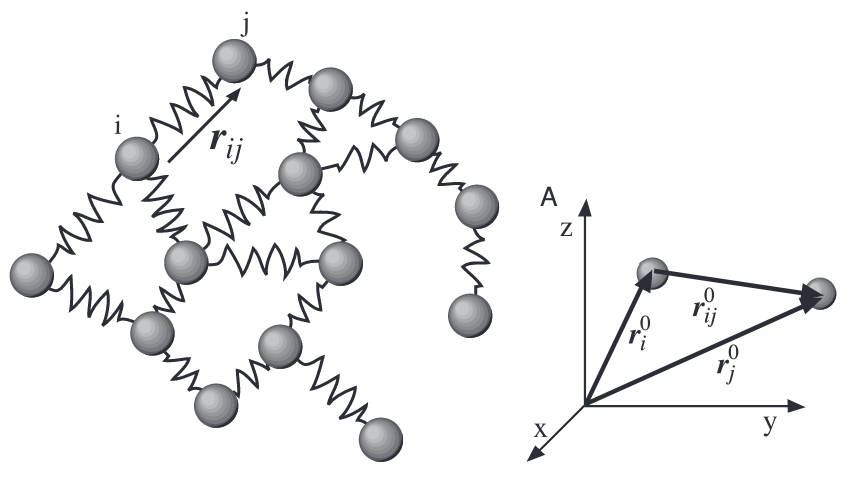
\includegraphics[width=8cm]{/home/michele_puppin/Scrivania/stesura_tesi/immagini/elastic_network.png}
	\caption{Raffigurazione del modello a rete elastica \cite{iop_science}}
	\label{fig:elastic_network}
\end{figure}

Per questo lavoro di tesi si è scelto di prendere in considerazione il modello anisotropo nel quale il potenziale scelto ha la forma 
\begin{equation} \label{eq:potential_anm}
	V = \frac{1}{2} \sum_{ij} \gamma_{ij} (R_{ij} -R_{ij}^{0} )^2.
\end{equation}
Il metodo è detto anisotropo in quanto osservando l'equazione (\ref{eq:potential_anm}) si nota che il potenziale è nullo se $ R_{ij} = R_{ij}^{0} $, indifferentemente dalla direzione dei corrispondenti vettori distanza. Con questo metodo risulta facile scrivere l'espressione della matrice $ \mathbf{H} $ utilizzando le equazioni (\ref{eq:potential_anm}) e (\ref{def_mat}). In questo caso la derivata seconda del potenziale è semplicemente
\begin{equation}
	\frac{\partial^2 V}{\partial x_i \: \partial y_j} = - \gamma_{ij} \frac{ (x_j - x_i) (y_j - y_i)}{R_{ij}^{2}}.
\end{equation}
Usando la notazione $ x_{ij}^0 = (x_{j}^{0}-x_{i}^{0}) $ per la prima componente del vettore distanza $ \mathbf{R}_{ij}^{0} $ e notazioni analoghe per $ y_{ij}^0 $ e $ z_{ij}^0 $, si possono scrivere le sottomatrici $ 3 \times 3 $ che si trovano fuori dalla diagonale di $ \mathbf{H} $ come
\begin{equation}\label{eq:sub_mat}
\mathbf{H}_{ij} = - \frac{\gamma_{ij}}{(R_{ij}^{0})^2} \left[
\begin{matrix}
(x_{ij}^0)^2 & x_{ij}^0 y_{ij}^0 & x_{ij}^0 z_{ij}^0\\
x_{ij}^0 y_{ij}^0 & (y_{ij}^0)^2 & y_{ij}^0 z_{ij}^0\\
x_{ij}^0z_{ij}^0 & y_{ij}^0 z_{ij}^0 & (z_{ij}^0)^2 \\
\end{matrix}
\right]
\end{equation}
mentre quelle sulla diagonale come 
\begin{equation}\label{eq:sub_mat_diag}
\mathbf{H}_{ii} = - \sum_{j;j\neq i} \mathbf{H}_{ij}.
\end{equation}

Con questo metodo è possibile generare conformazioni vicine alla struttura data deformandola lungo i modi dominanti. La configurazione deformata lungo il modo $ k $-esimo risulta essere 
\begin{equation}\label{eq:deformation}
	\mathbf{q}^{(k)} = 
	\mathbf{q}^0 \pm s \lambda_{k}^{-1/2} \mathbf{u}_{k}.
\end{equation}
Il parametro $ s $ dovrebbe scalare come $\sqrt{k_B	T}$.
La fluttuazione quadratica a temperatura $ T $ del residuo $ i $-esimo lungo un dato modo $ k $-esimo è data in termini dell'autovettore $ \mathbf{u}_{k} $ e dell'autovalore $ \lambda_k $ della matrice $ \mathbf{H} $ come 
\begin{equation}\label{eq:mob}
(\Delta \mathbf{R}_i)^2 \bigg|_k = k_B	T \: \mathrm{tr} \{[ \lambda_{k}^{-1} \mathbf{u}_{k} \mathbf{u}_{k}^{\mathrm{T}} ]_{ii}\} 
\end{equation}
e da conto della mobilità di un residuo lungo un determinato modo. Sommando su tutti i modi è possibile ottenere il coefficiente di mobilità che tiene conto della mobilità complessiva del residuo. Inoltre, poiché si è interessati in particolar modo alle deformazioni che riguardano ampie regioni della proteina, è utile andare a valutare quali modi presentino un grado di collettività più elevato. Il grado di collettività per una deformazione lungo il modo $ k $-esimo può essere valutato tramite il parametro $ \kappa_k $ definito come
\begin{equation}\label{eq:grado_coll}
	\kappa_k = \frac{1}{N} \exp \left( - \sum_{i=1}^{N} \alpha 	(\Delta \mathbf{R}_i)^2 \bigg|_k \log(\alpha (\Delta \mathbf{R}_i)^2)\bigg|_k \right)
\end{equation}
dove $ \alpha $ è la costante di normalizzazione tale per cui $ \sum_i \alpha (\Delta \mathbf{R}_i)^2 \lvert_k =1 $. \cite{chem_rev}
L'equazione (\ref{eq:grado_coll}) rappresenta l'entropia di Shannon definita come 
\begin{equation}
	S=- \sum_{i=1}^N p_i \ln p_i
\end{equation}
con $ p_i $ la probabilità di localizzazione del modo su ogni residuo. L'entropia sarà nulla qualora la deformazione risulti localizzata su un unico residuo, mentre assumerà il valore $ S= \ln N $ quando sarà massimamente distribuita su tutti gli $ N $ residui. Avendo definito il grado di collettività come $ \kappa_k = 1/N \exp (S)  $ si vede che questo avrà un valore minimo $ \kappa_k = 1/N $ (che per $ N \rightarrow \infty $ tenderà ad annullarsi) qualora $ S=0 $ e un valore massimo $ \kappa_k = 1 $ per $ S= \ln N $.
Si vede che il modo con il più alto grado di collettività avrà la più elevata entropia e sarà quindi distribuito su un maggior numero di residui.